\documentclass[11pt]{article}

\usepackage{float}
\usepackage{hyperref}
\usepackage{fullpage}
\usepackage{verbatim}
\usepackage{moreverb}
\usepackage{graphicx}
\usepackage{parskip}
\usepackage{amsmath}
\usepackage[toc,page]{appendix}

\usepackage{minted}
\let\verbatiminput=\verbatimtabinput
\def\verbatimtabsize{4\relax}

\begin{document}
\title{EE 241B HW1 Writeup}

\author{Vighnesh Iyer}
\date{}
\maketitle

\tableofcontents

\section{Models - MOSFET Characterization}

We are using a 32nm LP CMOS process for this class. The devices being characterized are \verb|n105| and \verb|p105| (TT corner) with a nominal supply voltage of 1.05V.

\subsection{Threshold Voltages}
We want to determine the threshold voltage $V_{th}$ for the NMOS and PMOS devices (for $V_{BS}$ = 0, $L$ = 32nm, and $W$ = 1$\mu$m), by extrapolating from the $I_DS$ vs. $V_{GS}$ curve at low $V_{DS}$. We compare the threshold voltage derived from DC sweeps to the values reported in the model file and the DC operating point analysis.

To perform this characterization, we first collect a full range of DC operating points for both transistors to make analysis easier for this entire section. The transistors' drains are connected to a variable DC supply and the transistors' gates are connected to another independent variable DC supply. The source for both transistors is held at ground or VDD (0V/1.5V). We perform a nested DC analysis by sweeping $V_{DS}$ from $0 \rightarrow 1.05$V in (10mV) increments, and sweep $V_{GS}$ from $0 \rightarrow 1.05$V in (10mV) increments.

The gathered I-V curves are shown below.

\begin{figure}[H]
	\centerline{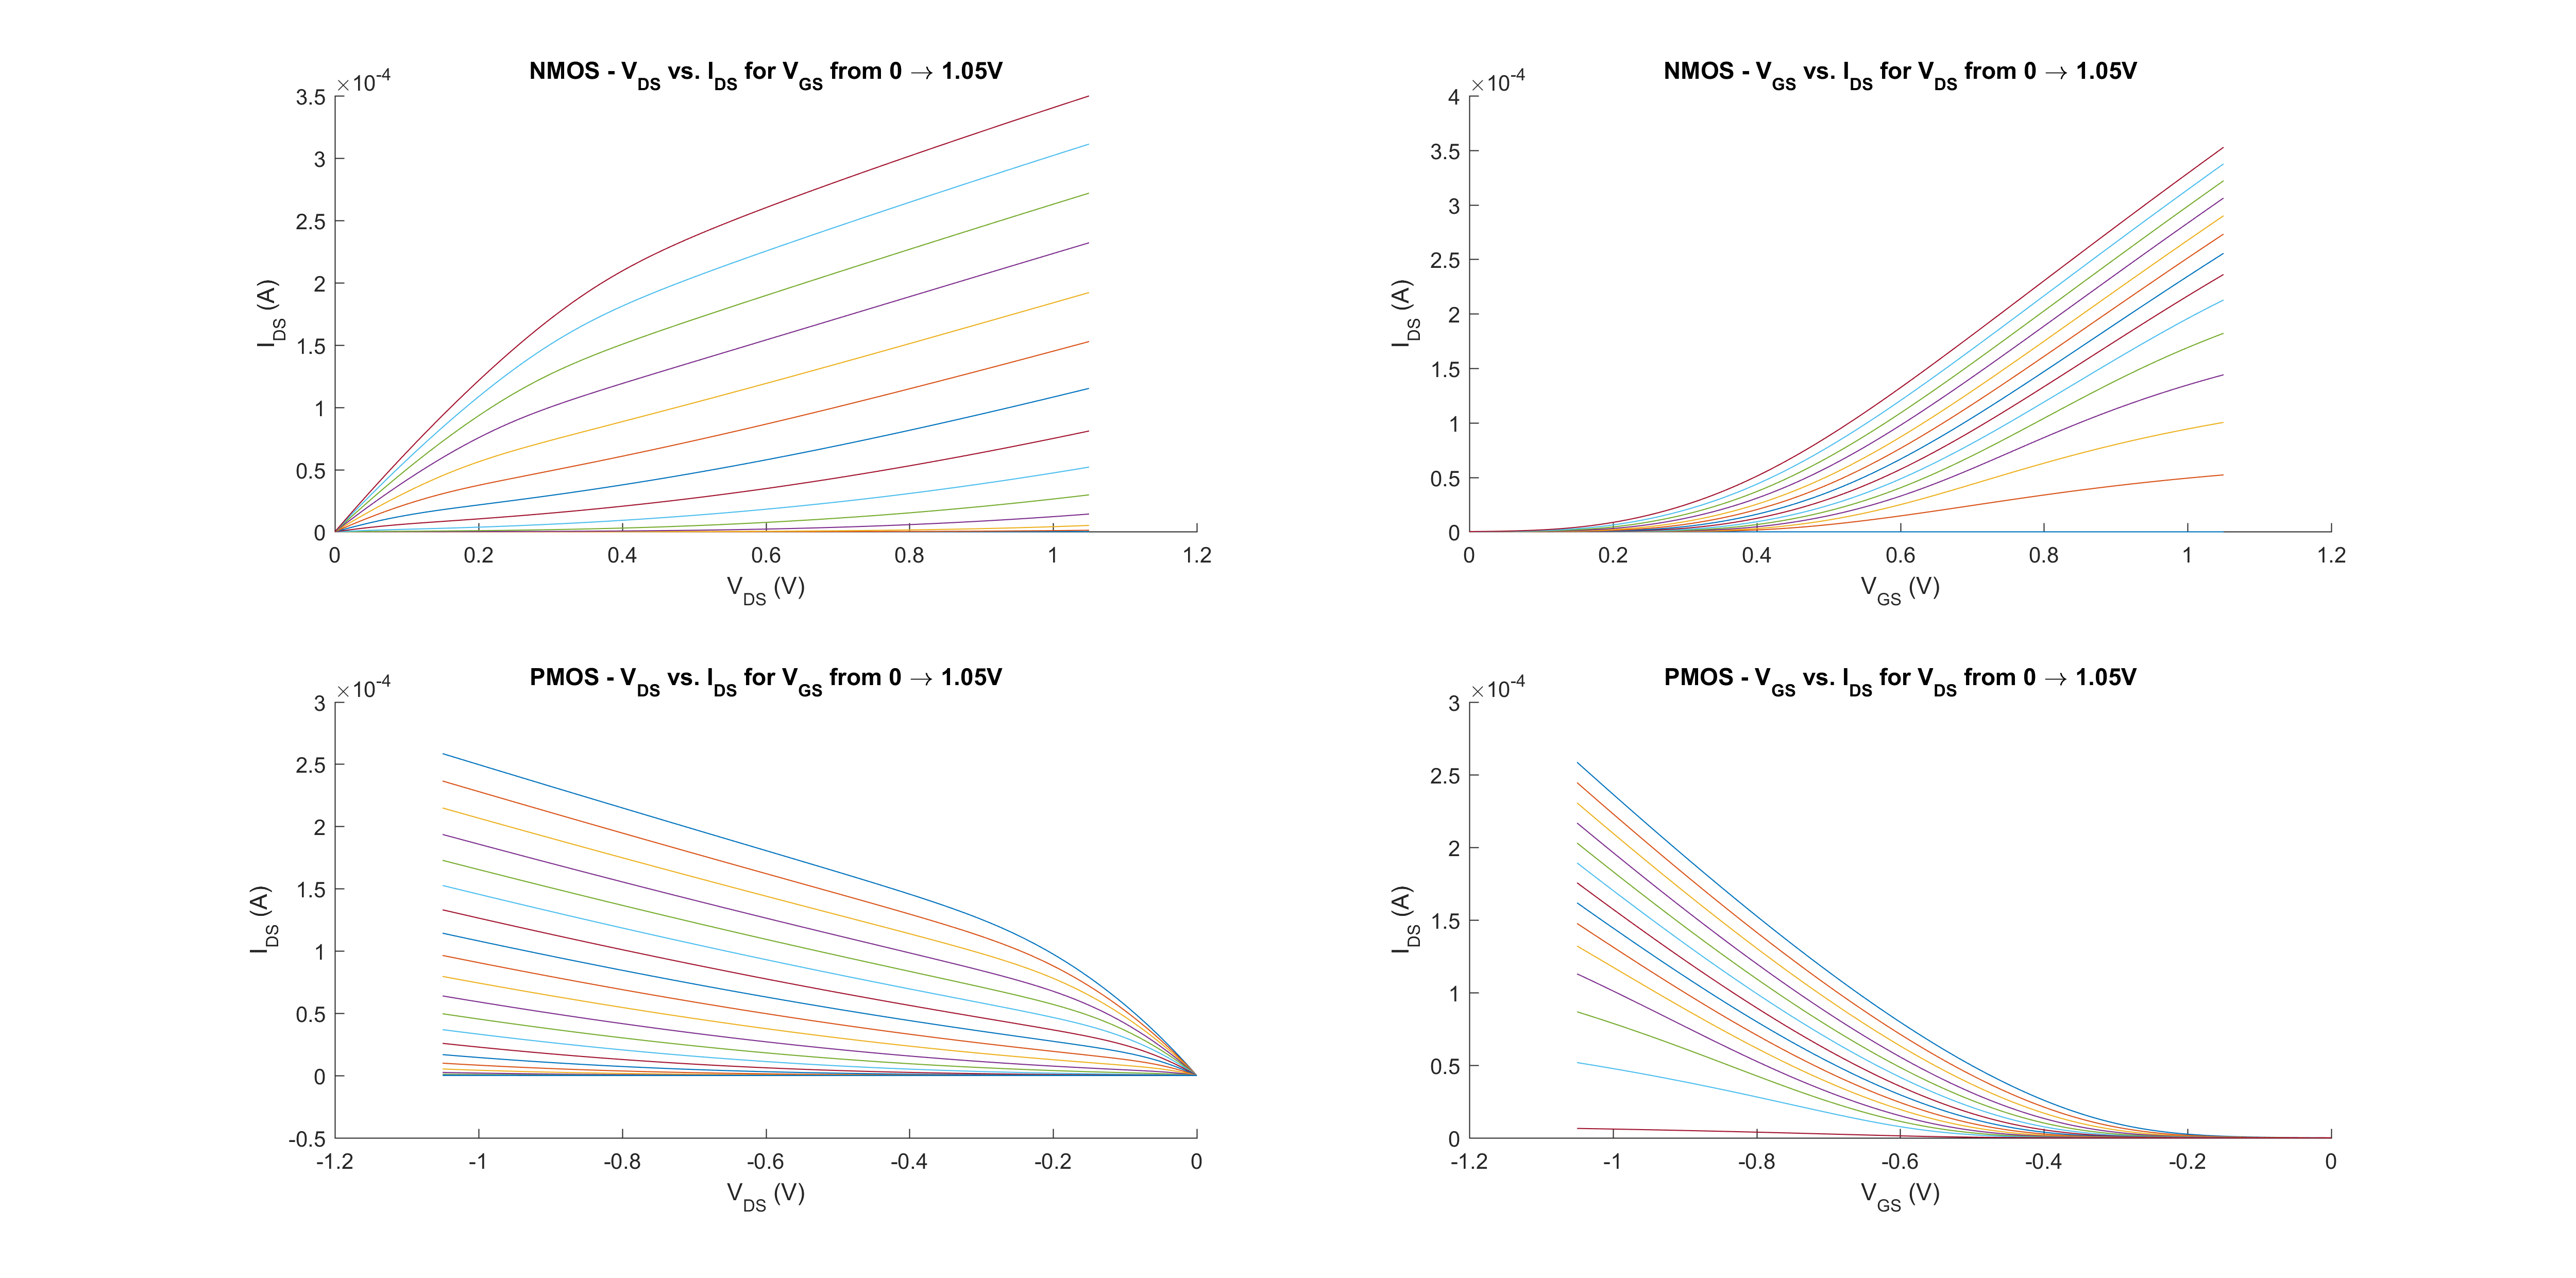
\includegraphics[width=\textwidth+5cm]{images/dc_curves.png}}	
\end{figure}

From the DC OP analysis, $V_{th}$ of the NMOS is reported to be 324.4 mV, and the $V_{th}$ of the PMOS is reported to be -208.1 mV. From the model files the NMOS $V_{th0}$ is 370 mV, and the PMOS $V_{th0}$ is -213 mV. However $V_{th0}$ is specified for long-channel devices, which don't accurately model the devices in this process.

To extract the threshold voltage from the I-V curves, we extrapolate the $V_{GS}$ vs $I_{DS}$ curves for a low value of $V_{DS}$ to keep the transistor in the linear region of operation. Then we fit a line to the linear part of the curves. We treat the x-intercept of those lines as the $V_{th}$ of the transistor for the selected value of $V_{DS}$. This method is shown for NMOS and PMOS transistors.

\begin{figure}[H]
	\centerline{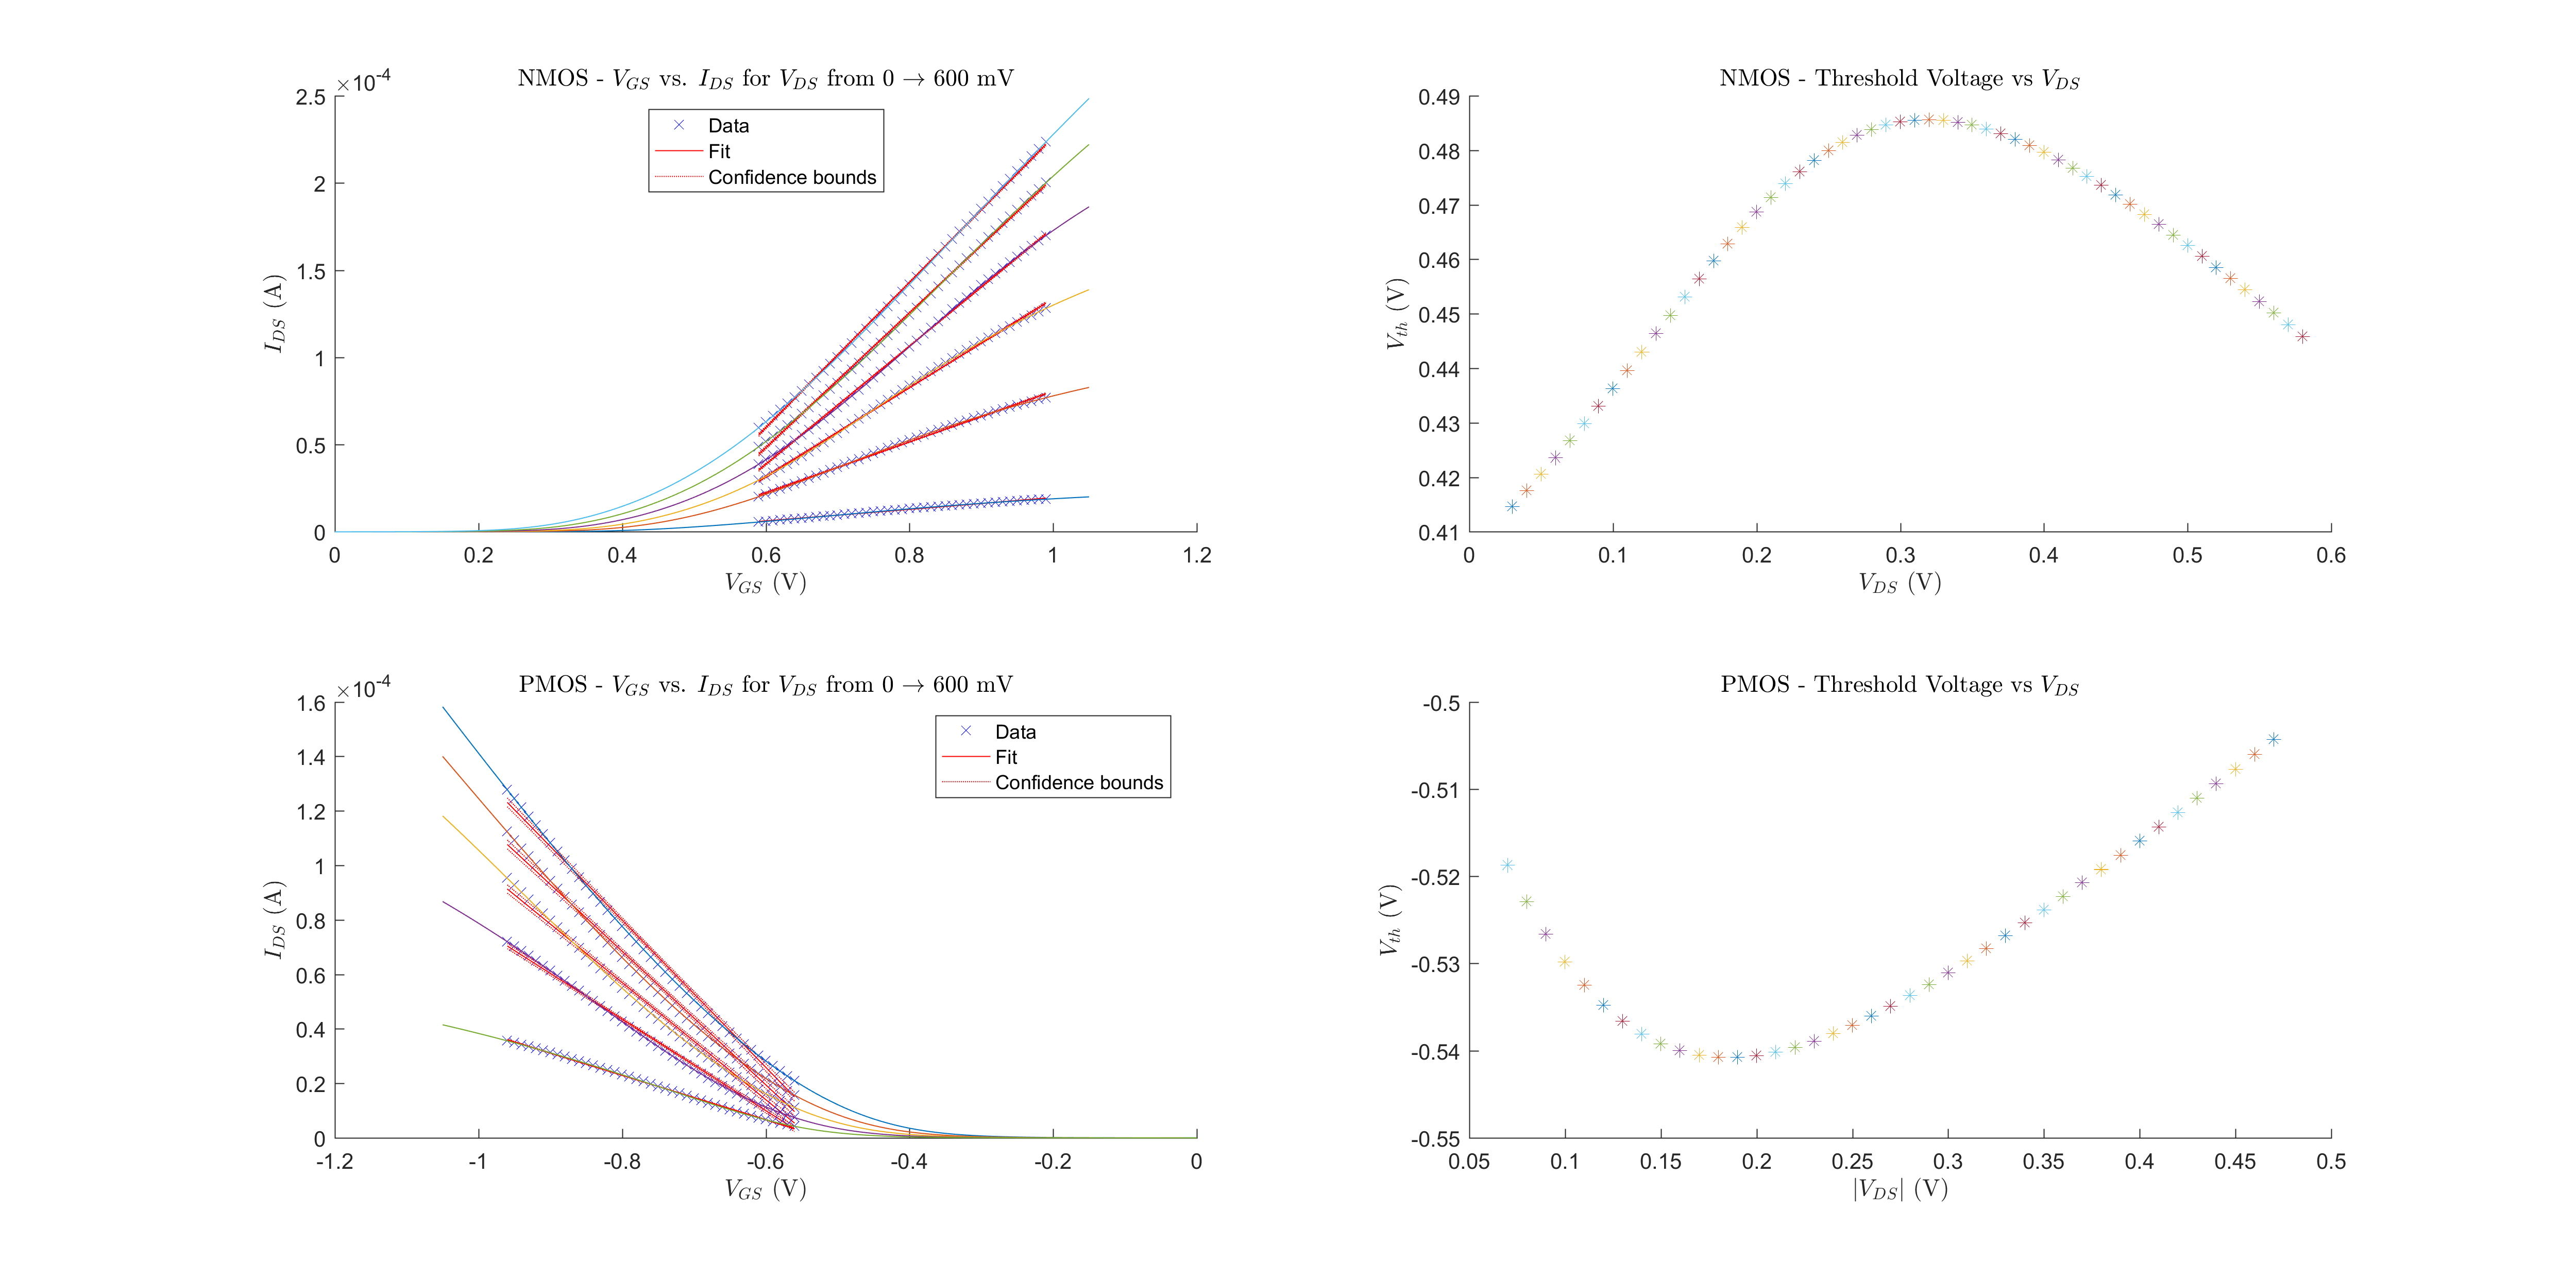
\includegraphics[width=\textwidth+5cm]{images/threshold_voltage.png}}	
\end{figure}

The images on the left side show the linear fit to each curve, while the images on the right side show the extrapolated $V_{th}$ for each $V_{DS}$ curve. As expected, with increased $V_{DS}$ the threshold voltage improves for both devices. 

The extrapolated results for the NMOS match the model files and the DC operating point measurement well. However, the PMOS threshold voltage is off by around 100 mV.

\subsection{Fitting Velocity Saturation Model}
In class, we use this model for $I_{DSat}$:

\begin{equation*}
	I_{DSat} = \frac{W}{L} \frac{\mu_{eff} C_{ox} E_C L}{2} \frac{(V_{GS} - V_{th})^2}{(V_{GS} - V_{th}) + E_C L}
\end{equation*}

We want to find the values of $E_C L$ that best fit the NMOS and PMOS I-V curves. We will use the $V_{th}$ value from the previous section. We take the case of the $V_{DS}$ curve where $V_{DS} = V_{DD}$ to keep the transistors fully saturated and we sweep $V_{GS}$. We then fit out data where $V_{GS} > V_{th}$ to this model with $E_C L$ and $k = \mu_{eff} C_{ox}$ as free variables.

To get starting values for fit iteration, I used model parameters to estimate $k$. $\frac{W}{L} = 31.25$. I found that for the NMOS $\mu_0$ (\verb|u0_n105|) is 30.4, $t_{ox}$ (\verb|toxe_n105|) is 2.39e-9, and $\epsilon_{ox}$ (\verb|epsrox|) is 3.9. For the PMOS $\mu_0$ (\verb|u0_p105|) is 60.95, $t_{ox}$ (\verb|toxe_p105|) is 2.62e-9, and $\epsilon_{ox}$ (\verb|epsrox|) is 3.9. We also know that $C_{ox} = \frac{\epsilon_{ox}}{t_{ox}}$.

Through experimentation, I found that $V_{th}$ from the previous section doesn't match this curve that well since the higher $V_{DS}$ results in a smaller effective threshold voltage. I then made $V_{th}$ another free variable to see if I could get a better fit.

After several iterations, it became clear that small changes in the initial guesses for the free variables resulted in very different curve fits. I settled on values that would give me a realistic $E_C L$ and $k$, but gave me a lower $V_{th}$ than expected.

\subsection{Fitting Alpha-Power Law}

\subsection{Fitting Alpha-Power Law ($\alpha = 1$)}

\section{Transistor Sizing}

\section{5-32 Decoder Design + VLSI Flow}

\subsection{GCD: VLSI's Hello World}

Here are the first 45 lines of the post-PAR Verilog netlist:
\begin{minted}[linenos]{verilog}
module gcdGCDUnitCtrl (clk , reset_BAR , operands_val , result_rdy , 
B_zero , A_lt_B , result_val , operands_rdy , A_mux_sel , B_mux_sel , 
A_en , B_en , IN0 );
input  clk ;
input  reset_BAR ;
input  operands_val ;
input  result_rdy ;
input  B_zero ;
input  A_lt_B ;
output result_val ;
output operands_rdy ;
output [1:0] A_mux_sel ;
output B_mux_sel ;
output A_en ;
output B_en ;
input  IN0 ;


wire [1:0] state ;

AND2X1_RVT icc_clock3 (.Y ( n16 ) , .A1 ( A_lt_B ) , .A2 ( n5 ) ) ;
NBUFFX8_RVT CTSNBUFFX32_RVT_G1B3I1 (.A ( clk_G1B5I1 ) , .Y ( clk_G1B6I1 ) ) ;
INVX2_RVT CTSINVX32_RVT_G1B13I1 (.A ( clk ) , .Y ( clk_G1B1I1 ) ) ;
NBUFFX8_RVT CTSNBUFFX2_RVT_G1B1I1 (.A ( clk_G1B6I1 ) , .Y ( clk_G1B7I1 ) ) ;
NBUFFX8_RVT CTSNBUFFX2_RVT_G1B5I1 (.A ( clk_G1B2I1 ) , .Y ( clk_G1B5I1 ) ) ;
INVX16_RVT CTSINVX32_RVT_G1B11I1 (.A ( clk_G1B1I1 ) , .Y ( clk_G1B2I1 ) ) ;
INVX0_RVT icc_place4 (.A ( n7 ) , .Y ( n10 ) ) ;
DELLN1X2_RVT icc_place3 (.A ( operands_val ) , .Y ( n7 ) ) ;
DFFX1_RVT state_reg_1_ (.QN ( n17 ) , .Q ( state[1] ) , .D ( n11 ) 
, .CLK ( clk_G1B7I1 ) ) ;
NAND2X0_RVT U24 (.A2 ( n14 ) , .A1 ( n15 ) , .Y ( A_en ) ) ;
INVX0_RVT U23 (.A ( B_en ) , .Y ( n15 ) ) ;
NAND4X0_RVT U22 (.A2 ( IN0 ) , .A4 ( n8 ) , .A3 ( n9 ) , .Y ( n11 ) , .A1 ( n13 ) ) ;
INVX0_RVT U21 (.A ( result_val ) , .Y ( n8 ) ) ;
NAND2X0_RVT U20 (.A2 ( state[1] ) , .A1 ( n10 ) , .Y ( n9 ) ) ;
NAND3X0_RVT U17 (.Y ( n13 ) , .A1 ( n6 ) , .A2 ( n5 ) , .A3 ( B_zero ) ) ;
AOI21X1_RVT U16 (.Y ( n12 ) , .A2 ( n3 ) , .A3 ( reset_BAR ) , .A1 ( n4 ) ) ;
NAND2X0_RVT U15 (.A2 ( state[0] ) , .A1 ( n2 ) , .Y ( n3 ) ) ;
NAND2X0_RVT U14 (.A2 ( state[1] ) , .A1 ( result_rdy ) , .Y ( n2 ) ) ;
NAND3X0_RVT U13 (.Y ( n4 ) , .A1 ( n6 ) , .A2 ( B_zero ) , .A3 ( n17 ) ) ;
INVX0_RVT U12 (.A ( A_lt_B ) , .Y ( n6 ) ) ;
AO21X1_RVT U11 (.A1 ( operands_rdy ) , .Y ( B_en ) , .A2 ( n7 ) , .A3 ( n16 ) ) ;
NOR2X0_RVT U10 (.Y ( A_mux_sel[1] ) , .A2 ( A_lt_B ) , .A1 ( n14 ) ) ;
OR2X1_RVT U9 (.Y ( n14 ) , .A2 ( B_zero ) , .A1 ( n1 ) ) ;
INVX0_RVT U8 (.A ( n5 ) , .Y ( n1 ) ) ;
AND2X2_RVT U7 (.Y ( operands_rdy ) , .A1 ( n18 ) , .A2 ( state[1] ) ) ;
\end{minted}

\begin{enumerate}
	\item Why are you generally not worried when you have hold time violations after synthesis?
	Hold time violations can be easily resolved later in the flow by inserting dummy logic/delay or by allowing a longer wire (with greater, non-zero delay) to connect the path that has a hold time violation.
	
	\item Why does the tutorial example (page 9) fail timing even though the delay is less than the clock period (0.5ns)?
	Even though the data arrival time is below 0.5ns, the data required time is also below 0.5ns, and to a greater extend than the data arrival time. This is due to factoring in the clock uncertainty (jitter/skew introduced later in the flow), and the setup time of the flip-flop.
	
	\item Why might you want to set a conservative \verb|clock_uncertainty|?
	A conservative \verb|clock_uncertainty| will account for any clock skew and jitter added during PAR. If the \verb|clock_uncertainty| is too optimistic, you may find that timing will pass when performing post-synthesis simulation, but will fail when trying post-PAR simulation.
\end{enumerate}

\subsection{Decoder Design}

Here is my decoder implementation in \verb|decoder.v|:

\begin{minted}[tabsize=2]{verilog}
module decoder(
	input [4:0] A,
	output reg [31:0] Z,
	input clk
);
	// NOTE: Testbench expects that the output Z is registered!
	genvar i;
	generate
		for (i = 0; i <= 5'd31; i = i + 1) begin:decoder_loop
			always @ (posedge clk) begin
				Z[i] <= A == i;
			end
		end
	endgenerate
endmodule
\end{minted}

I had to modify the `timescale in the \verb|decoder_tb| to be 1ns/10ps to match the vcd invocation and to ensure that a small clock period under 100ps would simulate without issues. The behavioral simulation succeeded.

After running \verb|dc-syn|, I found that there were timing violations, and I fixed those by increasing the clock period to 0.2ns. After this, I re-ran synthesis, verified that there were no timing violations, and ran the post-synthesis VCS sim to make sure the functionality of the decoder was still in order.

I then ran \verb|icc-par| and found several timing violations after PAR. They weren't internal to the decoder block, but rather involved the decoder's \verb|Z| register driving an output load capacitance of 30fF. This load capacitance is much higher than the internal capacitances in the circuit, so it takes a longer time to drive. The register needs to drive the output cap to its proper value before the next rising edge of the clock. I found that this will take at least 0.38ns, so I modified my clock period to 0.5ns to give the tools some slack.

After running post-PAR simulation, I found I needed to further increase the clock period to 1.0ns just to fix a testbench issue where the inputs to the decoder were supplied on the falling edge of the clock, rather than just right after the rising edge Clk-to-q to more accurately simulate the actual design.

Here are the final results:

\begin{enumerate}
	\item A screenshot of the layout
	\item Critical path in ns
	\item Post-PAR DVE sim showing correct functionality and critical path
\end{enumerate}
\newpage
\appendix
\section{PMOS/NMOS DC Characterization SPICE Sim} \label{dc_characterization_spice}
\begin{minted}{text}
Sweep of V_GS with constant V_DS for N-MOSFET
.lib '/home/ff/ee241/synopsys-32nm/hspice/saed32nm.lib' TT
vds vds gnd 1.05
vgs vgs gnd 1.05 
x1 vds vgs gnd gnd n105 (w=1u l=32n)

.op
.dc vgs 0 1.05 10m vds 0 1.05 10m

.option post=2 nomod
.end
\end{minted}

\section{}

\end{document}